\documentclass[pdftex,12pt, oneside]{article}

%\usepackage[paperwidth=8.5in, paperheight=13in]{geometry} % Folio
\usepackage[paperwidth=8.27in, paperheight=11.69in]{geometry} % A4

\usepackage{makeidx}         % allows index generation
\usepackage{graphicx}        % standard LaTeX graphics tool
                             % when including figure files
\usepackage[bottom]{footmisc}% places footnotes at page bottom
\usepackage[english]{babel}
\usepackage{enumerate}
\usepackage{paralist}
\usepackage{float}
\usepackage{gensymb}  
\usepackage{listings}
\usepackage{color}
\usepackage{mathtools} % atau \usepackage{amsmath}
\renewcommand{\baselinestretch}{1.5}

\newcommand{\HRule}{\rule{\linewidth}{0.5mm}}

\definecolor{codegreen}{rgb}{0,0.6,0}
\definecolor{codegray}{rgb}{0.5,0.5,0.5}
\definecolor{codepurple}{rgb}{0.58,0,0.82}
\definecolor{backcolor}{rgb}{0.95,0.95,0.92}

\lstdefinestyle{mystyle}{
  backgroundcolor=\color{backcolor},
  commentstyle=\color{codegreen},
  keywordstyle=\color{magenta},
  stringstyle=\color{codepurple},
  basicstyle=\footnotesize,
  breakatwhitespace=false,
  breaklines=true,
  captionpos=b,
  keepspaces=true,
  numbers=left,
  numbersep=5pt,
  showspaces=false,
  showstringspaces=false,
  showtabs=false,
  tabsize=2
}

\lstset{style=mystyle}


\begin{document}
\sloppy % biar section ga melebar melewati kertas

\begin{center}
{\large LAPORAN PELAKSANAAN UJI COBA PROGRAM - WS PBB}
\\[1cm]
xx Januari 2017\\
Priyanto Tamami, S.Kom.
\end{center}

%\frontmatter%%%%%%%%%%%%%%%%%%%%%%%%%%%%%%%%%%%%%%%%%%%%%%%%%%%%%%


%%%%%%%%%%%%%%%%%%%%%%%%%%%%%%%%%%%%%%%%%%%%%%%%%%%%%%%%%%%%%%%%%%%%%%

\section{PENDAHULUAN}

Pengujian program atau aplikasi yang dilakukan berupa \textit{unit testing} dan \textit{integration testing} menggunakan \textit{tools} yang sudah ada pada bahasa pemrograman Java yaitu JUnit.

JUnit ini nantinya akan melakukan testing per unit pada tiap fungsi / \textit{method} yang membangun sistem aplikasi sehingga diharapkan tiap unit menghasilkan keluaran yang diharapkan.

\section{OUTPUT PROGRAM}

Karena menggunakan JUnit, maka keluarannya akan menghasilkan informasi \texttt{fail} dan \texttt{passed}.

Kondisi pengujian seperti dijelaskan sebelumnya bahwa akan dilakukan dengan \textit{unit test} dan \textit{integration test}, rinciannya adalah sebagai berikut :

\begin{enumerate}[A.]
  \item \textit{Unit Test}
  
  \textit{Unit test} yang dilakukan akan dibagi berdasarkan kelas/objek yang terbentuk, berikut adalah nama \textit{file} yang melakukan \textit{unit test}, nama \textit{file} menunjukkan nama kelas/objek yang dilakukan \textit{unit test}.
  
  \begin{enumerate}[1.]
    \item RootControllerTest
    
    Pengujian kelas/objek \texttt{RootController} adalah untuk memastikan bahwa \textit{request} yang masuk ke \textit{server} mendapatkan respon yang diinginkan seperti nilai yang tertera pada basis data. Kode untuk melakukan pengujian pada kelas/objek \texttt{RootController} ini adalah sebagai berikut :
    
    \begin{lstlisting}
package lab.aikibo.controller;

import lab.aikibo.constant.StatusRespond;
import lab.aikibo.model.*;
import lab.aikibo.services.PembayaranServices;
import lab.aikibo.services.ReversalServices;
import lab.aikibo.services.SpptServices;
import org.joda.time.DateTime;
import org.junit.Before;
import org.junit.Test;
import org.junit.runner.RunWith;
import org.mockito.InjectMocks;
import org.mockito.Mock;
import org.mockito.Mockito;
import org.springframework.test.context.junit4.SpringRunner;

import javax.servlet.http.HttpServletRequest;
import java.math.BigInteger;

import static org.junit.Assert.assertEquals;
import static org.junit.Assert.assertNull;
import static org.mockito.Mockito.when;

/**
 * Created by tamami.
 */
@RunWith(SpringRunner.class)
public class RootControllerTest {

    @InjectMocks
    private RootController rootController = new RootController();

    HttpServletRequest mock = Mockito.mock(HttpServletRequest.class);

    @Mock
    private SpptServices spptServices;
    @Mock
    private PembayaranServices byrServices;
    @Mock
    private ReversalServices revServices;

    private StatusInq status;
    private StatusInq statusInqGagalDataTidakAda;
    private StatusInq statusInqError;
    private Sppt sppt;

    private StatusTrx statusTrxBerhasil;
    private StatusTrx statusTrxNihil;
    private StatusTrx statusTrxTerbayar;
    private StatusTrx statusTrxBatal;
    private StatusTrx statusTrxError;
    private StatusTrx statusTrxhnPajakBukanAngka;
    private StatusTrx statusTrxWaktuBayarLdWaktuCatat;
    private PembayaranSppt byrSppt;

    private StatusRev statusRevBerhasil;
    private StatusRev statusRevNihil;
    private StatusRev statusRevGanda;
    private StatusRev statusRevError;
    private ReversalPembayaran revSppt;

    @Before
    public void init() {
        sppt = new Sppt("332901000100100010", "2013", "FULAN", "BREBES",
                new BigInteger("10000"), new BigInteger("0"));
        status = new StatusInq(1, "Data Ditemukan", sppt);
        statusInqGagalDataTidakAda = new StatusInq(StatusRespond.DATA_INQ_NIHIL, "Data Tidak Ditemukan", null);
        statusInqError = new StatusInq(StatusRespond.DATABASE_ERROR, "Kesalahan DB", null);

        byrSppt = new PembayaranSppt("332901000100100010","2013","KODE_NTPD","4.1.1.12.1",
                new BigInteger("10000"), "4.1.1.12.2", new BigInteger("0"), "FULAN",
                "BREBES");
        statusTrxBerhasil = new StatusTrx(StatusRespond.APPROVED, "Pembayaran Telah Tercatat", byrSppt);
        statusTrxNihil = new StatusTrx(StatusRespond.TAGIHAN_TELAH_TERBAYAR,
                "Tagihan Telah Terbayar atau Pokok Pajak Nihil", null);
        statusTrxTerbayar = new StatusTrx(StatusRespond.TAGIHAN_TELAH_TERBAYAR,
                "Tagihan Telah Terbayar", null);
        statusTrxBatal = new StatusTrx(StatusRespond.JUMLAH_SETORAN_NIHIL,
                "Tagihan SPPT Telah Dibatalkan", null);
        statusTrxError = new StatusTrx(StatusRespond.DATABASE_ERROR,
                "Kesalahan Server", null);

        revSppt = new ReversalPembayaran("332901000100100010","2013","KODE_NTPD");
        statusRevBerhasil = new StatusRev(StatusRespond.APPROVED, "Proses Reversal Berhasil", revSppt);
        statusRevNihil = new StatusRev(StatusRespond.DATA_INQ_NIHIL, "Data Yang Diminta Tidak Ada", null);
        statusRevGanda = new StatusRev(StatusRespond.DATABASE_ERROR, "Data Tersebut Ganda", null);
        statusRevError = new StatusRev(StatusRespond.DATABASE_ERROR, "Kesalahan Server", null);
    }

    @Test
    public void testInquirySpptBerhasil() {
        when(spptServices.getSpptByNopThn("332901000100100010","2013",null))
                .thenReturn(status);

        assertEquals(1, rootController.getSppt("332901000100100010","2013", mock).getCode());
        assertEquals("Data Ditemukan",
                rootController.getSppt("332901000100100010", "2013", mock).getMessage());
        assertEquals("332901000100100010",
                rootController.getSppt("332901000100100010","2013", mock).getSppt().getNop());
        assertEquals("2013",
                rootController.getSppt("332901000100100010","2013", mock).getSppt().getThn());
        assertEquals("FULAN",
                rootController.getSppt("332901000100100010","2013", mock).getSppt().getNama());
        assertEquals("BREBES",
                rootController.getSppt("332901000100100010","2013", mock).getSppt().getAlamatOp());
        assertEquals(new BigInteger("10000"),
                rootController.getSppt("332901000100100010", "2013", mock).getSppt().getPokok());
        assertEquals(new BigInteger("0"),
                rootController.getSppt("332901000100100010", "2013", mock).getSppt().getDenda());
    }

    @Test
    public void testInquirySpptGagalKarnaNihil() {
        when(spptServices.getSpptByNopThn("332901000100100020","2013",null))
                .thenReturn(statusInqGagalDataTidakAda);

        assertEquals(10,
                rootController.getSppt("332901000100100020","2013", mock).getCode());
        assertEquals("Data Tidak Ditemukan",
                rootController.getSppt("332901000100100020","2013", mock).getMessage());
        assertNull(rootController.getSppt("332901000100100020","2013", mock).getSppt());
    }

    @Test
    public void testInquiryDbError() {
        when(spptServices.getSpptByNopThn("332901000100100030","2013",null))
                .thenReturn(statusInqError);

        assertEquals(4,
                rootController.getSppt("332901000100100030","2013", mock).getCode());
        assertEquals("Kesalahan DB",
                rootController.getSppt("332901000100100030","2013", mock).getMessage());
        assertNull(rootController.getSppt("332901000100100030","2013", mock).getSppt());
    }

    @Test
    public void testInquiryThnPajakBukanAngka() {
        assertEquals(36,
                rootController.getSppt("332901000100100010","2a13", mock).getCode());
        assertEquals("Tahun Pajak Mengandung Karakter Bukan Angka",
                rootController.getSppt("332901000100100010","2a13", mock).getMessage());
        assertNull(rootController.getSppt("332901000100100010","2a13", mock).getSppt());
    }

    @Test
    public void testTrxWaktuBayarLdWaktuCatat() {
        assertEquals(StatusRespond.TGL_JAM_BAYAR_LD_TGL_JAM_KIRIM,
                rootController.prosesPembayaran("332901000100100010","2013","22122017",
                        "1000", mock).getCode());
        assertEquals("Tanggal atau jam pada saat dibayarkan melebihi tanggal dan jam saat ini",
                rootController.prosesPembayaran("332901000100100010","2013","22122017",
                        "1000", mock).getMessage());
        assertNull(rootController.prosesPembayaran("332901000100100010","2013","22122017",
                "1000", mock).getByrSppt());
    }

    @Test
    public void testTrxSpptSukses() {
        when(byrServices.prosesPembayaran("332901000100100010","2013",
                new DateTime(2016, 12, 19, 10, 0),null))
                .thenReturn(statusTrxBerhasil);

        assertEquals(1,
                rootController.prosesPembayaran("332901000100100010","2013","19122016",
                        "1000", mock).getCode());
        assertEquals("Pembayaran Telah Tercatat",
                rootController.prosesPembayaran("332901000100100010","2013","19122016",
                        "1000", mock).getMessage());
        assertEquals("332901000100100010",
                rootController.prosesPembayaran("332901000100100010","2013","19122016",
                        "1000", mock).getByrSppt().getNop());
        assertEquals("2013",
                rootController.prosesPembayaran("332901000100100010","2013","19122016",
                        "1000", mock).getByrSppt().getThn());
        assertEquals("KODE_NTPD",
                rootController.prosesPembayaran("332901000100100010","2013","19122016",
                        "1000", mock).getByrSppt().getNtpd());
        assertEquals("4.1.1.12.1",
                rootController.prosesPembayaran("332901000100100010","2013","19122016",
                        "1000", mock).getByrSppt().getMataAnggaranPokok());
        assertEquals(new BigInteger("10000"),
                rootController.prosesPembayaran("332901000100100010","2013","19122016",
                        "1000", mock).getByrSppt().getPokok());
        assertEquals("4.1.1.12.2",
                rootController.prosesPembayaran("332901000100100010","2013","19122016",
                        "1000", mock).getByrSppt().getMataAnggaranSanksi());
        assertEquals(new BigInteger("0"),
                rootController.prosesPembayaran("332901000100100010", "2013","19122016",
                        "1000", mock).getByrSppt().getSanksi());
        assertEquals("FULAN",
                rootController.prosesPembayaran("332901000100100010", "2013", "19122016",
                        "1000", mock).getByrSppt().getNamaWp());
        assertEquals("BREBES",
                rootController.prosesPembayaran("332901000100100010","2013","19122016",
                        "1000", mock).getByrSppt().getAlamatOp());
    }



    @Test
    public void testTrxNihil() {
        when(byrServices.prosesPembayaran("332901000100100010","2013",
                new DateTime(2016, 12, 19, 10, 0),null))
                .thenReturn(statusTrxNihil);

        assertEquals(StatusRespond.TAGIHAN_TELAH_TERBAYAR,
                rootController.prosesPembayaran("332901000100100010","2013",
                        "19122016","1000", mock).getCode());
        assertEquals("Tagihan Telah Terbayar atau Pokok Pajak Nihil",
                rootController.prosesPembayaran("332901000100100010","2013","19122016",
                        "1000", mock).getMessage());
        assertNull(rootController.prosesPembayaran("332901000100100010","2013","19122016",
                "1000", mock).getByrSppt());
    }

    @Test
    public void testTrxTerbayar() {
        when(byrServices.prosesPembayaran("332901000100100010","2013",
                new DateTime(2016,12,19,10,0), null)).thenReturn(statusTrxTerbayar);

        assertEquals(StatusRespond.TAGIHAN_TELAH_TERBAYAR,
                rootController.prosesPembayaran("332901000100100010","2013","19122016",
                        "1000", mock).getCode());
        assertEquals("Tagihan Telah Terbayar",
                rootController.prosesPembayaran("332901000100100010","2013","19122016",
                        "1000", mock).getMessage());
        assertNull(rootController.prosesPembayaran("332901000100100010","2013","19122016",
                "1000", mock).getByrSppt());
    }

    @Test
    public void testTrxBatal() {
        when(byrServices.prosesPembayaran("332901000100100010","2013",
                new DateTime(2016,12,19,10,0), null)).thenReturn(statusTrxBatal);

        assertEquals(StatusRespond.JUMLAH_SETORAN_NIHIL,
                rootController.prosesPembayaran("332901000100100010","2013","19122016",
                        "1000", mock).getCode());
        assertEquals("Tagihan SPPT Telah Dibatalkan",
                rootController.prosesPembayaran("332901000100100010","2013","19122016",
                        "1000", mock).getMessage());
        assertNull(rootController.prosesPembayaran("332901000100100010","2013","19122016",
                "1000", mock).getByrSppt());
    }

    @Test
    public void testTrxError() {
        when(byrServices.prosesPembayaran("332901000100100010","2013",
                new DateTime(2016,12,19,10,0), null)).thenReturn(statusTrxError);

        assertEquals(StatusRespond.DATABASE_ERROR,
                rootController.prosesPembayaran("332901000100100010","2013","19122016",
                        "1000", mock).getCode());
        assertEquals("Kesalahan Server",
                rootController.prosesPembayaran("332901000100100010", "2013","19122016",
                        "1000", mock).getMessage());
        assertNull(rootController.prosesPembayaran("332901000100100010","2013","19122016",
                "1000", mock).getByrSppt());
    }

    @Test
    public void testRevSukses() {
        when(revServices.prosesReversal("332901000100100010","2013","KODE_NTPD", null))
                .thenReturn(statusRevBerhasil);

        assertEquals(StatusRespond.APPROVED,
                rootController.prosesReversal("332901000100100010","2013","KODE_NTPD", mock).getCode());
        assertEquals("Proses Reversal Berhasil",
                rootController.prosesReversal("332901000100100010","2013","KODE_NTPD", mock).getMessage());
        assertEquals("332901000100100010",
                rootController.prosesReversal("332901000100100010","2013","KODE_NTPD", mock)
                        .getRevPembayaran().getNop());
        assertEquals("2013",
                rootController.prosesReversal("332901000100100010","2013","KODE_NTPD", mock)
                        .getRevPembayaran().getThn());
        assertEquals("KODE_NTPD",
                rootController.prosesReversal("332901000100100010","2013","KODE_NTPD", mock)
                        .getRevPembayaran().getNtpd());
    }

    @Test
    public void testRevNihil() {
        when(revServices.prosesReversal("332901000100100010","2013","KODE_NTPD", null))
                .thenReturn(statusRevNihil);

        assertEquals(StatusRespond.DATA_INQ_NIHIL,
                rootController.prosesReversal("332901000100100010","2013","KODE_NTPD", mock).getCode());
        assertEquals("Data Yang Diminta Tidak Ada",
                rootController.prosesReversal("332901000100100010","2013","KODE_NTPD", mock).getMessage());
        assertNull(rootController.prosesReversal("332901000100100010","2013","KODE_NTPD", mock).
                getRevPembayaran());
    }

    @Test
    public void testRevGanda() {
        when(revServices.prosesReversal("332901000100100010","2013","KODE_NTPD", null))
                .thenReturn(statusRevGanda);

        assertEquals(StatusRespond.DATABASE_ERROR,
                rootController.prosesReversal("332901000100100010","2013","KODE_NTPD", mock).getCode());
        assertEquals("Data Tersebut Ganda",
                rootController.prosesReversal("332901000100100010","2013","KODE_NTPD", mock).getMessage());
        assertNull(rootController.prosesReversal("332901000100100010","2013","KODE_NTPD", mock)
                .getRevPembayaran());
    }

    @Test
    public void testRevError() {
        when(revServices.prosesReversal("332901000100100010","2013","KODE_NTPD", null))
                .thenReturn(statusRevError);

        assertEquals(StatusRespond.DATABASE_ERROR,
                rootController.prosesReversal("332901000100100010","2013","KODE_NTPD", mock).getCode());
        assertEquals("Kesalahan Server",
                rootController.prosesReversal("332901000100100010","2013","KODE_NTPD", mock).getMessage());
        assertNull(rootController.prosesReversal("332901000100100010","2013","KODE_NTPD", mock)
                .getRevPembayaran());
    }

}
    \end{lstlisting}
    
    Agar tidak mengganggu kondisi data pada sistem basis data yang berjalan, maka \textit{unit test} ini menggunakan data model sebagaimana disiapkan pada \textit{method} \texttt{init()}, kemudian datanya akan di \textit{mock} ke dalam \textit{service} yang menangani, seperti misalkan pada kasus \textit{inquiry} data SPPT, maka data model akan di \textit{mock} ke dalam objek \texttt{SpptServices}, yang apabila diujikan ada \textit{request} masuk melalui \textit{method} \texttt{getSppt}, maka seharusnya sistem akan menghasilkan data persis seperti apa yang telah di \textit{mock} ke dalam \textit{service}.
    
    Hasil dari \textit{unit test} tersebut seperti terlihat pada gambar \ref{fig:root-controller-ut}
    
    \begin{figure}[H]
      \centering
      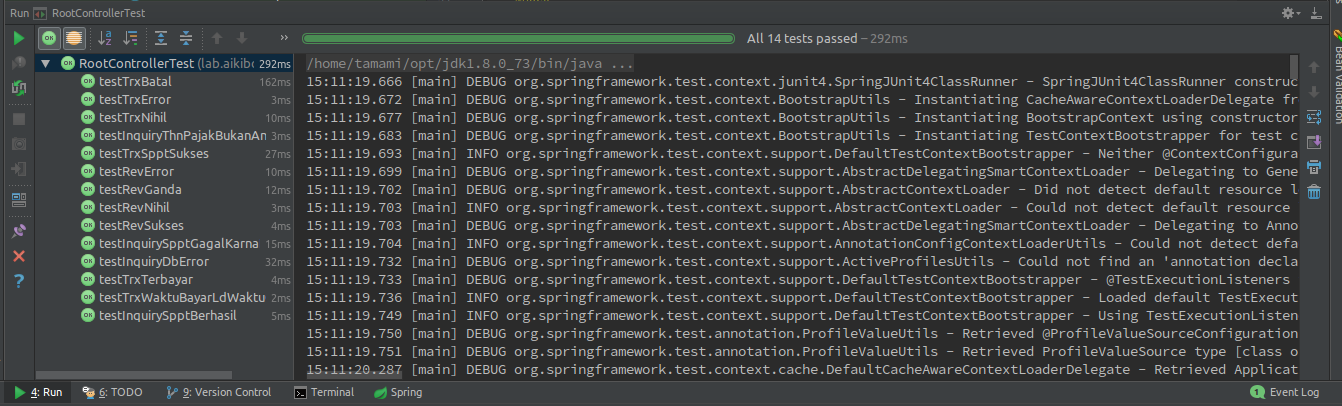
\includegraphics[width=1\textwidth]{./resources/01-root-controller-ut}
      \caption{Hasil \textit{Unit Test} Untuk Kelas \texttt{RootController}}
      \label{fig:root-controller-ut}
    \end{figure}
    
    Dari hasil tersebut menunjukkan bahwa pengujian telah berhasil dilakukan.
    
    \item StoreProceduresDaoImplTest
    
    Pengujian pada kelas \texttt{StoreProceduresDaoImplTest} dilakukan untuk memastikan bahwa proses di dalam kelas \texttt{StoreProceduresDaoImpl} berjalan sebagaimana seharusnya.
    
    Kode pengujian untuk kelas \texttt{StoreProceduresDaoImpl} ini adalah sebagai berikut :
    
    \begin{lstlisting}
package lab.aikibo.dao;

import lab.aikibo.constant.StatusRespond;
import lab.aikibo.model.*;
import org.joda.time.DateTime;
import org.junit.Before;
import org.junit.Test;
import org.mockito.Mock;
import org.mockito.Mockito;

import java.math.BigInteger;

import static org.junit.Assert.assertEquals;
import static org.junit.Assert.assertNull;
import static org.mockito.Mockito.when;

/**
 * Created by tamami.
 */
public class StoreProceduresDaoImplTest {

    @Mock
    private StoreProceduresDao spDao;

    private StatusInq statusInq;
    private StatusInq statusInqNihil;
    private StatusInq statusInqError;
    private Sppt sppt;

    private StatusTrx statusTrxBerhasil;
    private StatusTrx statusTrxNihil;
    private StatusTrx statusTrxTerbayar;
    private StatusTrx statusTrxBatal;
    private StatusTrx statusTrxError;
    private PembayaranSppt byrSppt;

    private StatusRev statusRevBerhasil;
    private StatusRev statusRevNihil;
    private StatusRev statusRevGanda;
    private StatusRev statusRevError;
    private ReversalPembayaran revSppt;


    @Before
    public void init() {
        spDao = Mockito.mock(StoreProceduresDaoImpl.class);

        sppt = new Sppt("332901000100100010", "2013", "FULAN", "BREBES",
                new BigInteger("10000"), new BigInteger("0"));
        statusInq = new StatusInq(StatusRespond.APPROVED, "Data Ditemukan", sppt);
        statusInqNihil = new StatusInq(StatusRespond.DATA_INQ_NIHIL, "Data Tidak Ditemukan", null);
        statusInqError = new StatusInq(StatusRespond.DATABASE_ERROR, "Kesalahan DB", null);

        byrSppt = new PembayaranSppt("332901000100100010","2013","KODE_NTPD","4.1.1.12.1",
                new BigInteger("10000"), "4.1.1.12.2", new BigInteger("0"), "FULAN",
                "BREBES");
        statusTrxBerhasil = new StatusTrx(StatusRespond.APPROVED, "Transaksi Telah Tercatat", byrSppt);
        statusTrxNihil = new StatusTrx(StatusRespond.JUMLAH_SETORAN_NIHIL, "Data Yang Diminta Tidak Ada",
                null);
        statusTrxTerbayar = new StatusTrx(StatusRespond.TAGIHAN_TELAH_TERBAYAR, "Tagihan Telah Terbayar", null);
        statusTrxBatal = new StatusTrx(StatusRespond.JUMLAH_SETORAN_NIHIL, "Tagihan Telah Dibatalkan", null);
        statusTrxError = new StatusTrx(StatusRespond.DATABASE_ERROR, "Kesalahan Server", null);

        revSppt = new ReversalPembayaran("332901000100100010","2013","KODE_NTPD");
        statusRevBerhasil = new StatusRev(StatusRespond.APPROVED, "Reversal Telah Berhasil Dilakukan", revSppt);
        statusRevNihil = new StatusRev(StatusRespond.DATA_INQ_NIHIL, "Data Yang Diminta Tidak Ada",
                null);
        statusRevGanda = new StatusRev(StatusRespond.DATABASE_ERROR, "Data Transaksi Tercatat Ganda",
                null);
        statusRevError = new StatusRev(StatusRespond.DATABASE_ERROR, "Kesalahan Server",
                null);
    }

    @Test
    public void testInqBerhasil() {
        when(spDao.getDataSppt("332901000100100010","2013", null))
                .thenReturn(statusInq);

        assertEquals(StatusRespond.APPROVED,
                spDao.getDataSppt("332901000100100010","2013",null).getCode());
        assertEquals("Data Ditemukan",
                spDao.getDataSppt("332901000100100010","2013", null).getMessage());
        assertEquals("332901000100100010",
                spDao.getDataSppt("332901000100100010","2013", null).getSppt().getNop());
        assertEquals("2013",
                spDao.getDataSppt("332901000100100010","2013", null).getSppt().getThn());
        assertEquals("FULAN",
                spDao.getDataSppt("332901000100100010","2013", null).getSppt().getNama());
        assertEquals("BREBES",
                spDao.getDataSppt("332901000100100010","2013", null).getSppt().getAlamatOp());
        assertEquals(new BigInteger("10000"),
                spDao.getDataSppt("332901000100100010","2013", null).getSppt().getPokok());
        assertEquals(new BigInteger("0"),
                spDao.getDataSppt("332901000100100010","2013", null).getSppt().getDenda());
    }

    @Test
    public void testInqNihil() {
        when(spDao.getDataSppt("332901000100100010","2013",null))
                .thenReturn(statusInqNihil);

        assertEquals(StatusRespond.DATA_INQ_NIHIL,
                spDao.getDataSppt("332901000100100010","2013",null).getCode());
        assertEquals("Data Tidak Ditemukan",
                spDao.getDataSppt("332901000100100010","2013", null).getMessage());
        assertNull(spDao.getDataSppt("332901000100100010","2013", null).getSppt());
    }

    @Test
    public void testInqError() {
        when(spDao.getDataSppt("332901000100100010", "2013", null))
                .thenReturn(statusInqError);

        assertEquals(StatusRespond.DATABASE_ERROR,
                spDao.getDataSppt("332901000100100010","2013", null).getCode());
        assertEquals("Kesalahan DB",
                spDao.getDataSppt("332901000100100010","2013", null).getMessage());
        assertNull(spDao.getDataSppt("332901000100100010","2013",null).getSppt());
    }

    @Test
    public void testTrxSukses() {
        when(spDao.prosesPembayaran("332901000100100010","2013",
                new DateTime(2016,12,19,10,0).toDate(), null))
                .thenReturn(statusTrxBerhasil);

        assertEquals(StatusRespond.APPROVED,
                spDao.prosesPembayaran("332901000100100010","2013",
                        new DateTime(2016,12,19,10,0).toDate(), null).getCode());
        assertEquals("Transaksi Telah Tercatat",
                spDao.prosesPembayaran("332901000100100010","2013",
                        new DateTime(2016,12,19,10,0).toDate(), null).getMessage());
        assertEquals("332901000100100010",
                spDao.prosesPembayaran("332901000100100010","2013",
                        new DateTime(2016,12,19,10,0).toDate(), null).getByrSppt().getNop());
        assertEquals("2013",
                spDao.prosesPembayaran("332901000100100010","2013",
                        new DateTime(2016,12,19,10,0).toDate(), null).getByrSppt().getThn());
        assertEquals("KODE_NTPD",
                spDao.prosesPembayaran("332901000100100010","2013",
                        new DateTime(2016,12,19,10,0).toDate(), null).getByrSppt().getNtpd());
        assertEquals("4.1.1.12.1",
                spDao.prosesPembayaran("332901000100100010","2013",
                        new DateTime(2016,12,19,10,0).toDate(), null).getByrSppt()
                        .getMataAnggaranPokok());
        assertEquals(new BigInteger("10000"),
                spDao.prosesPembayaran("332901000100100010","2013",
                        new DateTime(2016,12,19,10,0).toDate(), null).getByrSppt()
                        .getPokok());
        assertEquals("4.1.1.12.2",
                spDao.prosesPembayaran("332901000100100010","2013",
                        new DateTime(2016,12,19,10,0).toDate(), null).getByrSppt()
                        .getMataAnggaranSanksi());
        assertEquals(new BigInteger("0"),
                spDao.prosesPembayaran("332901000100100010","2013",
                        new DateTime(2016,12,19,10,0).toDate(), null).getByrSppt().getSanksi());
        assertEquals("FULAN",
                spDao.prosesPembayaran("332901000100100010","2013",
                        new DateTime(2016,12,19,10,0).toDate(), null).getByrSppt().getNamaWp());
        assertEquals("BREBES",
                spDao.prosesPembayaran("332901000100100010","2013",
                        new DateTime(2016,12,19,10,0).toDate(), null).getByrSppt().getAlamatOp());
    }

    @Test
    public void testTrxNihil() {
        when(spDao.prosesPembayaran("332901000100100010","2013",
                new DateTime(2016,12,19,10,0).toDate(), null))
                .thenReturn(statusTrxNihil);

        assertEquals(StatusRespond.JUMLAH_SETORAN_NIHIL,
                spDao.prosesPembayaran("332901000100100010","2013",
                        new DateTime(2016,12,19,10,0).toDate(), null).getCode());
        assertEquals("Data Yang Diminta Tidak Ada",
                spDao.prosesPembayaran("332901000100100010","2013",
                        new DateTime(2016,12,19,10,0).toDate(), null).getMessage());
        assertNull(spDao.prosesPembayaran("332901000100100010","2013",
                new DateTime(2016,12,19,10,0).toDate(), null).getByrSppt());
    }

    @Test
    public void testTrxTerbayar() {
        when(spDao.prosesPembayaran("332901000100100010","2013",
                new DateTime(2016,12,19,10,0).toDate(), null))
                .thenReturn(statusTrxTerbayar);

        assertEquals(StatusRespond.TAGIHAN_TELAH_TERBAYAR,
                spDao.prosesPembayaran("332901000100100010","2013",
                        new DateTime(2016,12,19,10,0).toDate(), null).getCode());
        assertEquals("Tagihan Telah Terbayar",
                spDao.prosesPembayaran("332901000100100010","2013",
                        new DateTime(2016,12,19,10,0).toDate(), null).getMessage());
        assertNull(spDao.prosesPembayaran("332901000100100010","2013",
                        new DateTime(2016,12,19,10,0).toDate(), null).getByrSppt());
    }

    @Test
    public void testTrxBatal() {
        when(spDao.prosesPembayaran("332901000100100010","2013",
                new DateTime(2016,12,19,10,0).toDate(), null))
                .thenReturn(statusTrxBatal);

        assertEquals(StatusRespond.JUMLAH_SETORAN_NIHIL,
                spDao.prosesPembayaran("332901000100100010","2013",
                        new DateTime(2016,12,19,10,00).toDate(),null).getCode());
        assertEquals("Tagihan Telah Dibatalkan",
                spDao.prosesPembayaran("332901000100100010","2013",
                        new DateTime(2016,12,19,10,0).toDate(), null).getMessage());
        assertNull(spDao.prosesPembayaran("332901000100100010","2013",
                        new DateTime(2016,12,19,10,0).toDate(), null).getByrSppt());
    }

    @Test
    public void testTrxError() {
        when(spDao.prosesPembayaran("332901000100100010","2013",
                new DateTime(2016,12,19,10,0).toDate(), null))
                .thenReturn(statusTrxError);

        assertEquals(StatusRespond.DATABASE_ERROR,
                spDao.prosesPembayaran("332901000100100010","2013",
                        new DateTime(2016,12,19,10,0).toDate(), null).getCode());
        assertEquals("Kesalahan Server",
                spDao.prosesPembayaran("332901000100100010","2013",
                        new DateTime(2016,12,19,10,0).toDate(), null).getMessage());
        assertNull(spDao.prosesPembayaran("332901000100100010","2013",
                new DateTime(2016,12,19,10,0).toDate(), null).getByrSppt());
    }

    @Test
    public void testRevSukses() {
        when(spDao.reversalPembayaran("332901000100100010","2013","KODE_NTPD", null))
                .thenReturn(statusRevBerhasil);

        assertEquals(StatusRespond.APPROVED,
                spDao.reversalPembayaran("332901000100100010","2013","KODE_NTPD", null).getCode());
        assertEquals("Reversal Telah Berhasil Dilakukan",
                spDao.reversalPembayaran("332901000100100010", "2013", "KODE_NTPD", null).getMessage());
        assertEquals("332901000100100010",
                spDao.reversalPembayaran("332901000100100010","2013", "KODE_NTPD", null)
            .getRevPembayaran().getNop());
        assertEquals("2013",
                spDao.reversalPembayaran("332901000100100010","2013","KODE_NTPD", null)
                        .getRevPembayaran().getThn());
        assertEquals("KODE_NTPD",
                spDao.reversalPembayaran("332901000100100010","2013", "KODE_NTPD", null)
                        .getRevPembayaran().getNtpd());

    }

    @Test
    public void testRevNihil() {
        when(spDao.reversalPembayaran("332901000100100010","2013","KODE_NTPD", null))
                .thenReturn(statusRevNihil);

        assertEquals(StatusRespond.DATA_INQ_NIHIL,
                spDao.reversalPembayaran("332901000100100010","2013","KODE_NTPD", null)
                        .getCode());
        assertEquals("Data Yang Diminta Tidak Ada",
                spDao.reversalPembayaran("332901000100100010","2013","KODE_NTPD", null)
                        .getMessage());
        assertNull(spDao.reversalPembayaran("332901000100100010","2013","KODE_NTPD", null)
                .getRevPembayaran());
    }

    @Test
    public void testRevDouble() {
        when(spDao.reversalPembayaran("332901000100100010","2013","KODE_NTPD", null))
                .thenReturn(statusRevGanda);

        assertEquals(StatusRespond.DATABASE_ERROR,
                spDao.reversalPembayaran("332901000100100010","2013","KODE_NTPD", null)
                        .getCode());
        assertEquals("Data Transaksi Tercatat Ganda",
                spDao.reversalPembayaran("332901000100100010","2013","KODE_NTPD", null)
                        .getMessage());
        assertNull(spDao.reversalPembayaran("332901000100100010","2013","KODE_NTPD", null)
                .getRevPembayaran());
    }

    @Test
    public void testRevError() {
        when(spDao.reversalPembayaran("332901000100100010","2013","KODE_NTPD", null))
                .thenReturn(statusRevError);

        assertEquals(StatusRespond.DATABASE_ERROR,
                spDao.reversalPembayaran("332901000100100010","2013","KODE_NTPD", null)
                        .getCode());
        assertEquals("Kesalahan Server",
                spDao.reversalPembayaran("332901000100100010","2013","KODE_NTPD",null)
                        .getMessage());
        assertNull(spDao.reversalPembayaran("332901000100100010","2013","KODE_NTPD",null)
                .getRevPembayaran());
    }

}
    \end{lstlisting}
    
    Karena kelas \texttt{StoreProceduresDao} berkomunikasi langsung dengan sistem basis data, tugas \textit{unit test} ini adalah melakukan pengujian bahwa proses yang dihasilkan sesuai dengan isi basis data tanpa menyentuh atau berhubungan dengan sistem basis data, oleh karena itu pengujian pada kelas/objek \texttt{StoreProceduresDaoImplTest} menggunakan \textit{mocking} untuk membuat data model.
    
    Dari hasil pengujian tersebut, didapatkan hasil seperti terlihat pada gambar \ref{fig:sp-ut}
    
    \begin{figure}[H]
      \centering
      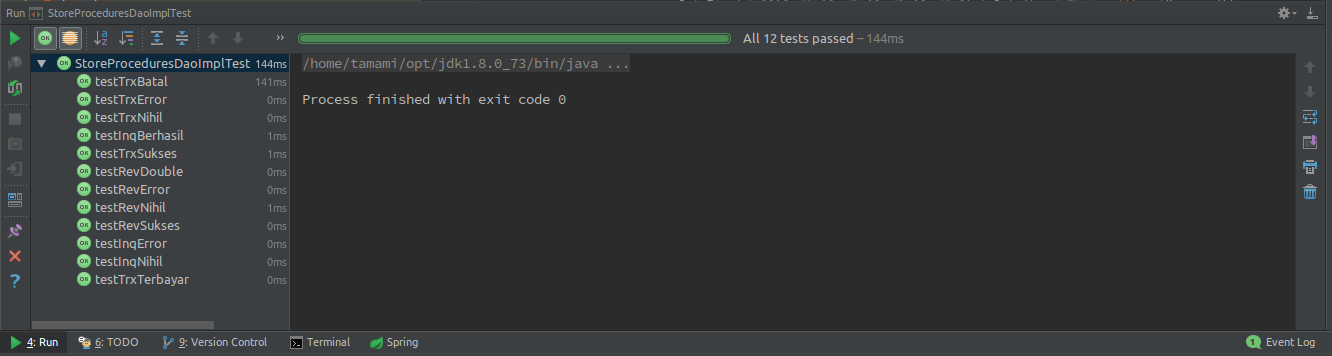
\includegraphics[width=1\textwidth]{./resources/02-sp-ut}
      \caption{Hasil \textit{Unit Test} Pada Kelas \texttt{StoreProceduresDaoImpl}}
      \label{fig:sp-ut}
    \end{figure}
    
    Dari gambar tersebut menunjukkan bahwa hasil pengujian yang dilakukan berhasil sesuai dengan apa yang diharapkan.
    
    \item PembayaranServicesImplTest
    
    Kelas/objek \texttt{PembayaranServicesImplTest} digunakan untuk melakukan pengujian pada kelas \texttt{PembayaranServicesImpl} yang menghubungkan bagian \textit{view} dan \textit{model} pada konsep MVC. Perlu dipastikan bahwa hasil dari pengambilan data pada sistem basis data diterima dengan benar oleh kelas/objek \texttt{RootController}, berikut adalah kode untuk melakukan \textit{unit testing} pada kelas \texttt{PembayaranServicesImplTest} :
    
    \begin{lstlisting}
package lab.aikibo.services;

import lab.aikibo.constant.StatusRespond;
import lab.aikibo.dao.StoreProceduresDaoImpl;
import lab.aikibo.model.PembayaranSppt;
import lab.aikibo.model.StatusTrx;
import org.joda.time.DateTime;
import org.junit.Before;
import org.junit.Test;
import org.junit.runner.RunWith;
import org.mockito.InjectMocks;
import org.mockito.Mock;
import org.springframework.test.context.junit4.SpringRunner;

import java.math.BigInteger;

import static org.junit.Assert.assertEquals;
import static org.junit.Assert.assertNull;
import static org.mockito.Mockito.when;

/**
 * Created by tamami.
 */
@RunWith(SpringRunner.class)
public class PembayaranServicesImplTest {

    @InjectMocks
    private PembayaranServicesImpl byrServices = new PembayaranServicesImpl();

    @Mock
    private StoreProceduresDaoImpl spDao;

    private StatusTrx statusTrxBerhasil;
    private StatusTrx statusTrxNihil;
    private StatusTrx statusTrxTerbayar;
    private StatusTrx statusTrxBatal;
    private StatusTrx statusTrxError;
    private StatusTrx statusTrxhnPajakBukanAngka;
    private StatusTrx statusTrxWaktuBayarLdWaktuCatat;
    private PembayaranSppt byrSppt;

    @Before
    public void init() {
        byrSppt = new PembayaranSppt("332901000100100010","2013","KODE_NTPD","4.1.1.12.1",
                new BigInteger("10000"), "4.1.1.12.2", new BigInteger("0"), "FULAN",
                "BREBES");
        statusTrxBerhasil = new StatusTrx(StatusRespond.APPROVED, "Transaksi Telah Tercatat", byrSppt);
        statusTrxNihil = new StatusTrx(StatusRespond.JUMLAH_SETORAN_NIHIL, "Data Yang Diminta Tidak Ada",
                null);
        statusTrxTerbayar = new StatusTrx(StatusRespond.TAGIHAN_TELAH_TERBAYAR, "Tagihan Telah Terbayar", null);
        statusTrxBatal = new StatusTrx(StatusRespond.JUMLAH_SETORAN_NIHIL, "Tagihan Telah Dibatalkan", null);
        statusTrxError = new StatusTrx(StatusRespond.DATABASE_ERROR, "Kesalahan Server", null);
    }

    @Test
    public void testTrxBerhasil() {
        when(spDao.prosesPembayaran("332901000100100010","2013",
                new DateTime(2016,12,20,10,0).toDate(), null)).thenReturn(statusTrxBerhasil);

        assertEquals(StatusRespond.APPROVED,
                byrServices.prosesPembayaran("332901000100100010","2013",
                        new DateTime(2016,12,20,10,0), null).getCode());
        assertEquals("Transaksi Telah Tercatat",
                byrServices.prosesPembayaran("332901000100100010","2013",
                        new DateTime(2016,12,20,10,0), null).getMessage());
        assertEquals("332901000100100010",
                byrServices.prosesPembayaran("332901000100100010","2013",
                        new DateTime(2016,12,20,10,0), null).getByrSppt().getNop());
        assertEquals("2013",
                byrServices.prosesPembayaran("332901000100100010","2013",
                        new DateTime(2016,12,20,10,0), null).getByrSppt().getThn());
        assertEquals("KODE_NTPD",
                byrServices.prosesPembayaran("332901000100100010","2013",
                        new DateTime(2016,12,20,10,0), null).getByrSppt().getNtpd());
        assertEquals("4.1.1.12.1",
                byrServices.prosesPembayaran("332901000100100010","2013",
                        new DateTime(2016,12,20,10,0),null).getByrSppt().getMataAnggaranPokok());
        assertEquals(new BigInteger("10000"),
                byrServices.prosesPembayaran("332901000100100010","2013",
                        new DateTime(2016,12,20,10,0),null).getByrSppt().getPokok());
        assertEquals("4.1.1.12.2",
                byrServices.prosesPembayaran("332901000100100010","2013",
                        new DateTime(2016,12,20,10,0), null).getByrSppt().getMataAnggaranSanksi());
        assertEquals(new BigInteger("0"),
                byrServices.prosesPembayaran("332901000100100010","2013",
                        new DateTime(2016,12,20,10,0), null).getByrSppt().getSanksi());
        assertEquals("FULAN",
                byrServices.prosesPembayaran("332901000100100010","2013",
                        new DateTime(2016,12,20,10,0),null).getByrSppt().getNamaWp());
        assertEquals("BREBES",
                byrServices.prosesPembayaran("332901000100100010","2013",
                        new DateTime(2016,12,20,10,0),null).getByrSppt().getAlamatOp());

    }

    @Test
    public void testTrxNihil() {
        when(spDao.prosesPembayaran("332901000100100010","2013",
                new DateTime(2016,12,20,10,0).toDate(), null)).thenReturn(statusTrxNihil);

        assertEquals(StatusRespond.JUMLAH_SETORAN_NIHIL,
                byrServices.prosesPembayaran("332901000100100010","2013",
                        new DateTime(2016,12,20,10,0), null).getCode());
        assertEquals("Data Yang Diminta Tidak Ada",
                byrServices.prosesPembayaran("332901000100100010","2013",
                        new DateTime(2016,12,20,10,0), null).getMessage());
        assertNull(byrServices.prosesPembayaran("332901000100100010","2013",
                new DateTime(2016,12,20,10,0),null).getByrSppt());
    }

    @Test
    public void testTrxTerbayar() {
        when(spDao.prosesPembayaran("332901000100100010","2013",
                new DateTime(2016,12,20,10,0).toDate(), null)).thenReturn(statusTrxTerbayar);

        assertEquals(StatusRespond.TAGIHAN_TELAH_TERBAYAR,
                byrServices.prosesPembayaran("332901000100100010","2013",
                        new DateTime(2016,12,20,10,0),null).getCode());
        assertEquals("Tagihan Telah Terbayar",
                byrServices.prosesPembayaran("332901000100100010","2013",
                        new DateTime(2016,12,20,10,0), null).getMessage());
        assertNull(byrServices.prosesPembayaran("332901000100100010","2013",
                new DateTime(2016,12,20,10,0), null).getByrSppt());
    }

    @Test
    public void testTrxBatal() {
        when(spDao.prosesPembayaran("332901000100100010","2013",
                new DateTime(2016,12,20,10,0).toDate(), null)).thenReturn(statusTrxBatal);

        assertEquals(StatusRespond.JUMLAH_SETORAN_NIHIL,
                byrServices.prosesPembayaran("332901000100100010","2013",
                        new DateTime(2016,12,20,10,0), null).getCode());
        assertEquals("Tagihan Telah Dibatalkan",
                byrServices.prosesPembayaran("332901000100100010","2013",
                        new DateTime(2016,12,20,10,0),null).getMessage());
        assertNull(byrServices.prosesPembayaran("332901000100100010","2013",
                new DateTime(2016,12,20,10,0), null).getByrSppt());
    }

    @Test
    public void testTrxError() {
        when(spDao.prosesPembayaran("332901000100100010","2013",
                new DateTime(2016,12,20,10,0).toDate(), null)).thenReturn(statusTrxError);

        assertEquals(StatusRespond.DATABASE_ERROR,
                byrServices.prosesPembayaran("332901000100100010","2013",
                        new DateTime(2016,12,20,10,0), null).getCode());
        assertEquals("Kesalahan Server",
                byrServices.prosesPembayaran("332901000100100010","2013",
                        new DateTime(2016,12,20,10,0), null).getMessage());
        assertNull(byrServices.prosesPembayaran("332901000100100010","2013",
                new DateTime(2016,12,20,10,0),null).getByrSppt());
    }

}
    \end{lstlisting}
    
    Seperti pada pengujian sebelumnya, pengujian kali ini pun tidak akan menggunakan data langsung dari sistem basis data, hanya dibuatkan modelnya sebagai simulasi.
    
    Hasil dari pengujian di atas adalah seperti terlihat pada gambar \ref{fig:byr-service-ut} :
    
    \begin{figure}[H]
      \centering
      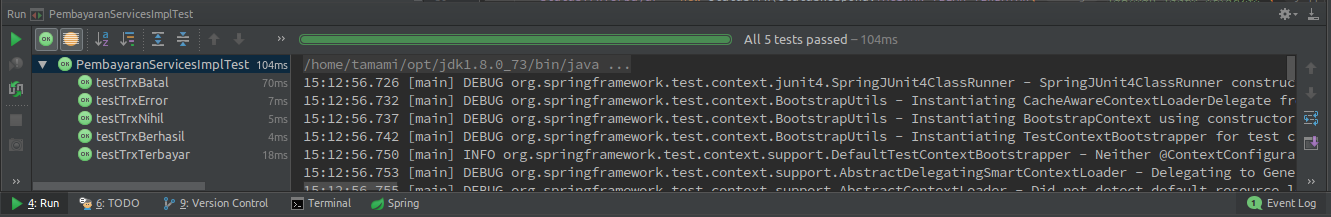
\includegraphics[width=1\textwidth]{./resources/03-byr-service-ut}
      \caption{Hasil \textit{Unit Test} Untuk kelas PembayaranServicesImpl}
      \label{fig:byr-service-ut}
    \end{figure}
    
    Dari gambar di atas menunjukkan bahwa pengujian telah dilakukan dan memberikan hasil sesuai dengan yang diharapkan.
    
    \item ReversalServicesImplTest
    
    Kelas \texttt{ReversalServicesImplTest} akan melakukan pengujian untuk kelas/objek \texttt{ReversalServicesImpl} yang menghubungkan antara kelas/objek \texttt{RootController} untuk fungsi reversal pembayaran. Berikut adalah kode lengkap dari kelas \texttt{ReversalServicesImplTest} :
    
    \begin{lstlisting}
package lab.aikibo.services;

import lab.aikibo.constant.StatusRespond;
import lab.aikibo.dao.StoreProceduresDaoImpl;
import lab.aikibo.model.ReversalPembayaran;
import lab.aikibo.model.StatusRev;
import org.junit.Before;
import org.junit.Test;
import org.junit.runner.RunWith;
import org.mockito.InjectMocks;
import org.mockito.Mock;
import org.springframework.test.context.junit4.SpringRunner;

import static org.junit.Assert.assertEquals;
import static org.junit.Assert.assertNull;
import static org.mockito.Mockito.when;

/**
 * Created by tamami.
 */
@RunWith(SpringRunner.class)
public class ReversalServicesImplTest {

    @InjectMocks
    private ReversalServicesImpl revServices = new ReversalServicesImpl();

    @Mock
    private StoreProceduresDaoImpl spDao;

    private StatusRev statusRevBerhasil;
    private StatusRev statusRevNihil;
    private StatusRev statusRevGanda;
    private StatusRev statusRevError;
    private ReversalPembayaran revSppt;

    @Before
    public void init() {
        revSppt = new ReversalPembayaran("332901000100100010","2013","KODE_NTPD");
        statusRevBerhasil = new StatusRev(StatusRespond.APPROVED, "Reversal Telah Berhasil Dilakukan", revSppt);
        statusRevNihil = new StatusRev(StatusRespond.DATA_INQ_NIHIL, "Data Yang Diminta Tidak Ada",
                null);
        statusRevGanda = new StatusRev(StatusRespond.DATABASE_ERROR, "Data Transaksi Tercatat Ganda",
                null);
        statusRevError = new StatusRev(StatusRespond.DATABASE_ERROR, "Kesalahan Server",
                null);
    }

    @Test
    public void testRevBerhasil() {
        when(spDao.reversalPembayaran("332901000100100010","2013","KODE_NTPD", null))
                .thenReturn(statusRevBerhasil);

        assertEquals(StatusRespond.APPROVED,
                revServices.prosesReversal("332901000100100010","2013","KODE_NTPD",null).getCode());
        assertEquals("Reversal Telah Berhasil Dilakukan",
                revServices.prosesReversal("332901000100100010","2013","KODE_NTPD", null).getMessage());
        assertEquals("332901000100100010",
                revServices.prosesReversal("332901000100100010","2013","KODE_NTPD",null)
                        .getRevPembayaran().getNop());
        assertEquals("2013",
                revServices.prosesReversal("332901000100100010","2013","KODE_NTPD",null)
                        .getRevPembayaran().getThn());
        assertEquals("KODE_NTPD",
                revServices.prosesReversal("332901000100100010","2013","KODE_NTPD",null)
                        .getRevPembayaran().getNtpd());
    }

    @Test
    public void testRevNihil() {
        when(spDao.reversalPembayaran("332901000100100010","2013","KODE_NTPD",null))
                .thenReturn(statusRevNihil);

        assertEquals(StatusRespond.DATA_INQ_NIHIL,
                revServices.prosesReversal("332901000100100010","2013","KODE_NTPD",null)
                        .getCode());
        assertEquals("Data Yang Diminta Tidak Ada",
                revServices.prosesReversal("332901000100100010","2013","KODE_NTPD",null)
                        .getMessage());
        assertNull(revServices.prosesReversal("332901000100100010","2013","KODE_NTPD",null)
                .getRevPembayaran());
    }

    @Test
    public void testRevGanda(){
        when(spDao.reversalPembayaran("332901000100100010","2013","KODE_NTPD",null))
                .thenReturn(statusRevGanda);

        assertEquals(StatusRespond.DATABASE_ERROR,
                revServices.prosesReversal("332901000100100010","2013","KODE_NTPD",null)
                        .getCode());
        assertEquals("Data Transaksi Tercatat Ganda",
                revServices.prosesReversal("332901000100100010","2013","KODE_NTPD",null)
                        .getMessage());
        assertNull(revServices.prosesReversal("332901000100100010","2013","KODE_NTPD",null)
                        .getRevPembayaran());
    }

    /**
     * @TODO: buat unit test untuk skenario reversal gagal karena kesalahan DB
     */
    @Test
    public void testRevError() {
        when(spDao.reversalPembayaran("332901000100100010","2013","KODE_NTPD",null))
                .thenReturn(statusRevError);

        assertEquals(StatusRespond.DATABASE_ERROR,
                revServices.prosesReversal("332901000100100010","2013","KODE_NTPD",null)
                        .getCode());
        assertEquals("Kesalahan Server",
                revServices.prosesReversal("332901000100100010","2013","KODE_NTPD", null)
                        .getMessage());
        assertNull(revServices.prosesReversal("332901000100100010","2013","KODE_NTPD",null)
                        .getRevPembayaran());
    }

}   
    \end{lstlisting}
    
    \textit{Unit test} dilakukan untuk setiap skenario yang memungkinkan terjadinya aksi, sehingga kelas ini mampu untuk melakukan tugasnya sebagai penghubung antara kelas/objek \textit{view} dan kelas/objek \textit{model} untuk fungsi reversal pembayaran.
    
    Hasil dari eksekusi kode di atas adalah seperti pada gambar \ref{fig:rev-service-ut} :
    
    \begin{figure}[H]
      \centering
      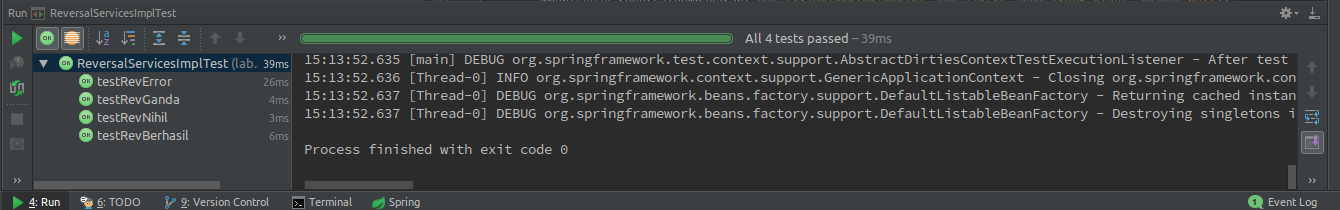
\includegraphics[width=1\textwidth]{./resources/04-rev-service-ut}
      \caption{Hasil \textit{Unit Test} terhadap kelas \texttt{ReversalServicesImpl}}
      \label{fig:rev-service-ut}
    \end{figure}
    
    Terlihat bahwa pengujian terhadap kelas/objek \texttt{ReversalServicesImpl} berhasil sepenuhnya.
    
    \item SpptServicesImplTest
    
    Kelas/objek ini akan melakukan \textit{unit test} pada kelas/objek \textit{SpptServicesImpl} untuk fungsi \textit{inquiry} data SPPT. Berikut adalah kode \textit{unit test} untuk kelas \texttt{SpptServicesImplTest} :
    
    \begin{lstlisting}
package lab.aikibo.services;

import lab.aikibo.constant.StatusRespond;
import lab.aikibo.dao.StoreProceduresDaoImpl;
import lab.aikibo.model.Sppt;
import lab.aikibo.model.StatusInq;
import org.junit.Before;
import org.junit.Test;
import org.junit.runner.RunWith;
import org.mockito.InjectMocks;
import org.mockito.Mock;
import org.springframework.test.context.junit4.SpringRunner;

import java.math.BigInteger;

import static org.junit.Assert.assertEquals;
import static org.junit.Assert.assertNull;
import static org.mockito.Mockito.when;

/**
 * Created by tamami.
 */
@RunWith(SpringRunner.class)
public class SpptServicesImplTest {

    @InjectMocks
    private SpptServicesImpl spptServices = new SpptServicesImpl();

    @Mock
    private StoreProceduresDaoImpl spDao;

    private StatusInq statusSukses;
    private StatusInq statusInqGagalDataTidakAda;
    private StatusInq statusInqError;
    private Sppt sppt;

    @Before
    public void init() {
        sppt = new Sppt("332901000100100010", "2013", "FULAN", "BREBES",
                new BigInteger("10000"), new BigInteger("0"));
        statusSukses = new StatusInq(1, "Data Ditemukan", sppt);
        statusInqGagalDataTidakAda = new StatusInq(StatusRespond.DATA_INQ_NIHIL, "Data Tidak Ditemukan", null);
        statusInqError = new StatusInq(StatusRespond.DATABASE_ERROR, "Kesalahan DB", null);
    }

    @Test
    public void testInqSukses() {
        when(spDao.getDataSppt("332901000100100010","2013",null)).thenReturn(statusSukses);

        assertEquals(StatusRespond.APPROVED,
                spptServices.getSpptByNopThn("332901000100100010","2013",null).getCode());
        assertEquals("Data Ditemukan",
                spptServices.getSpptByNopThn("332901000100100010","2013",null).getMessage());
        assertEquals("332901000100100010",
                spptServices.getSpptByNopThn("332901000100100010","2013",null).getSppt().getNop());
        assertEquals("2013",
                spptServices.getSpptByNopThn("332901000100100010","2013",null).getSppt().getThn());
        assertEquals("FULAN",
                spptServices.getSpptByNopThn("332901000100100010","2013",null).getSppt().getNama());
        assertEquals("BREBES",
                spptServices.getSpptByNopThn("332901000100100010","2013",null).getSppt().getAlamatOp());
        assertEquals(new BigInteger("10000"),
                spptServices.getSpptByNopThn("332901000100100010","2013",null).getSppt().getPokok());
        assertEquals(new BigInteger("0"),
                spptServices.getSpptByNopThn("332901000100100010","2013",null).getSppt().getDenda());
    }

    /**
     * @TODO: unit testing untuk skenario inquiry nihil
     */
    @Test
    public void testInqNihil() {
        when(spDao.getDataSppt("332901000100100010","2013",null)).thenReturn(statusInqGagalDataTidakAda);

        assertEquals(StatusRespond.DATA_INQ_NIHIL,
                spptServices.getSpptByNopThn("332901000100100010","2013",null).getCode());
        assertEquals("Data Tidak Ditemukan",
                spptServices.getSpptByNopThn("332901000100100010","2013",null).getMessage());
        assertNull(spptServices.getSpptByNopThn("332901000100100010","2013",null).getSppt());
    }

    /**
     * @TODO: unit testing untuk skenario inquiry error server
     */
    @Test
    public void testInqError() {
        when(spDao.getDataSppt("332901000100100010","2013",null)).thenReturn(statusInqError);

        assertEquals(StatusRespond.DATABASE_ERROR,
                spptServices.getSpptByNopThn("332901000100100010","2013",null).getCode());
        assertEquals("Kesalahan DB",
                spptServices.getSpptByNopThn("332901000100100010","2013",null).getMessage());
        assertNull(spptServices.getSpptByNopThn("332901000100100010","2013",null).getSppt());
    }

}
    \end{lstlisting}
    
    Pengujian kali ini pun menggunakan data model atau \textit{mock} untuk memastikan bahwa proses yang terjadi menghasilkan keluaran yang diinginkan.
    
    Hasil dari pengujian di atas adalah seperti terlihat pada gambar \ref{fig:inq-service-ut} :
    
    \begin{figure}[H]
      \centering
      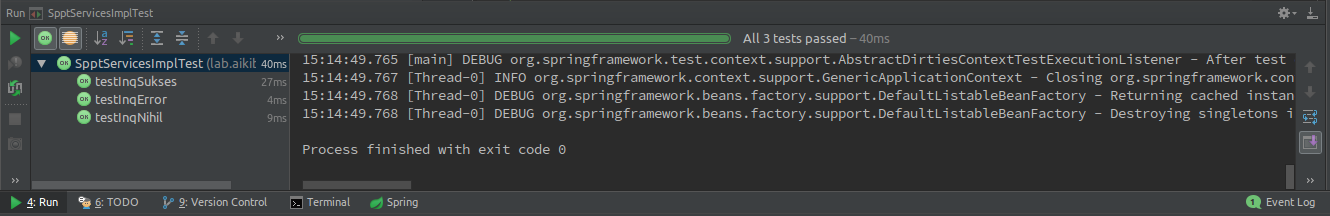
\includegraphics[width=1\textwidth]{./resources/05-inq-service-ut}
      \caption{Hasil \textit{Unit Test} untuk kelas \texttt{SpptServicesImpl}}
      \label{fig:inq-service-ut}
    \end{figure}
    
    Dari gambar tersebut di atas terlihat bahwa pengujian telah berhasil melakukan \textit{unit test} pada tiap kasus.
    
  \end{enumerate}
  
  \item \textit{Integration Test}
  
  \textit{Integration test} akan melakukan tugasnya untuk menguji apakah koneksi dengan sistem basis data berjalan sebagaimana yang diharapkan, \textit{integration test} yang dilakukan hanya akan dibagi menjadi 2 (dua) bagian, yaitu :
  
  \begin{enumerate}[1.]
    \item HibernateConfigurationIT
    
    \textit{Integration test} yang dilakukan kelas ini hanya untuk memastikan parameter yang digunakan untuk melakukan koneksi ke sistem basis data sudah benar, karena parameter yang digunakan disimpan dalam bentuk \textit{file} terpisah. Berikut adalah kode untuk melakukan integrasi terhadap \textit{file} konfigurasi sistem basis data :
    
    \begin{lstlisting}
package lab.aikibo.config;

import com.jolbox.bonecp.BoneCPDataSource;
import lab.aikibo.App;
import org.junit.Test;
import org.junit.runner.RunWith;
import org.springframework.beans.factory.annotation.Autowired;
import org.springframework.boot.test.context.SpringBootTest;
import org.springframework.test.context.junit4.SpringRunner;

import static org.junit.Assert.assertEquals;
import static org.junit.Assert.assertNotNull;

/**
 * Created by tamami.
 */
@RunWith(SpringRunner.class)
@SpringBootTest(classes=App.class)
public class HibernateConfigurationIT {

    @Autowired
    private BoneCPDataSource boneDS;

    /**
     * check driver
     */
    @Test
    public void testDriver() {
        assertEquals("oracle.jdbc.driver.OracleDriver", boneDS.getDriverClass());
    }

    /**
     * check jdbc url
     */
    @Test
    public void testJdbcDriver() {
        assertEquals("jdbc:oracle:thin:pbbdummy/pbbdummy@192.168.2.7:1521/sismiopbck", boneDS.getJdbcUrl());
    }

    /**
     * check db username
     */
    @Test
    public void testUsername() {
        assertEquals("pbbdummy", boneDS.getUsername());
    }

    /**
     * check db password
     */
    @Test
    public void testPassword() {
        assertEquals("pbbdummy", boneDS.getPassword());
    }

    /**
     * check db connection
     */
    @Test
    public void testDbConnection() {
        assertNotNull(boneDS);
    }

}
    \end{lstlisting}
    
    Hasil keluaran dari \textit{integration test} untuk kelas \texttt{HibernateConfigurationIT} adalah seperti terlihat pada gambar \ref{fig:06-hibernate-config-it} :
    
    \begin{figure}[H]
      \centering
      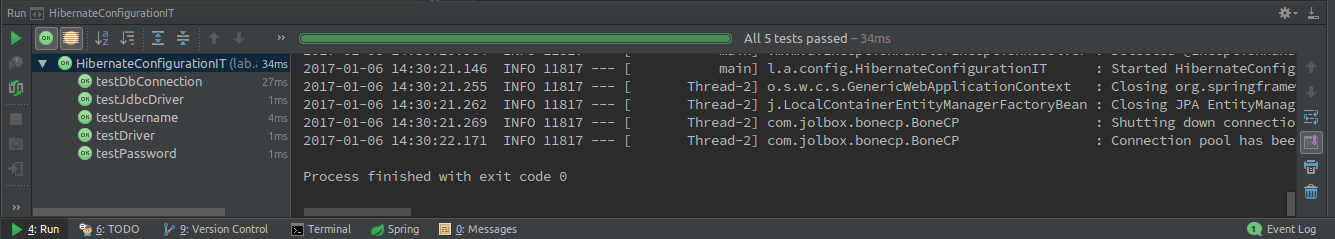
\includegraphics[width=1\textwidth]{./resources/06-hibernate-config-IT}
      \caption{Hasil \textit{Integration Test File} Konfigurasi Sistem Basis Data}
      \label{fig:06-hibernate-config-it}
    \end{figure}
    
    Terlihat bahwa dari 5 (lima) pengujian yang dilakukan sudah dapat memenuhi kualifikasi yang benar.
    
    \item ServicesIT
    
    Kelas \texttt{ServicesIT} ini akan melakukan \textit{integration test} terhadap kelas \textit{services} yang hubungannya langsung melakukan aksesnya pada sistem basis data. Agar tidak mengganggu sistem yang sedang berjalan, sistem basis data pun menggunakan model data yang sama persis sebagaimana sistem basis data yang digunakan pada fase produksi, yaitu menggunakan sistem basis data Oracle 11g.
    
    Berikut adalah kode untuk melakukan pengujian tersebut :
    
    \begin{lstlisting}
package lab.aikibo.services;

import lab.aikibo.App;
import lab.aikibo.constant.StatusRespond;
import lab.aikibo.model.StatusInq;
import lab.aikibo.model.StatusRev;
import lab.aikibo.model.StatusTrx;
import org.joda.time.DateTime;
import org.junit.Test;
import org.junit.runner.RunWith;
import org.springframework.beans.factory.annotation.Autowired;
import org.springframework.boot.test.context.SpringBootTest;
import org.springframework.test.context.junit4.SpringRunner;

import java.math.BigInteger;

import static org.junit.Assert.assertEquals;

/**
 * Created by tamami.
 */
@RunWith(SpringRunner.class)
@SpringBootTest(classes=App.class)
public class ServicesIT {

    @Autowired
    private SpptServices spptServices;

    @Autowired
    private PembayaranServices byrServices;

    @Autowired
    private ReversalServices revServices;

    @Test
    public void testInquiry() {
        StatusInq statusInq = spptServices.getSpptByNopThn("332901000100100010","2013","192.168.2.1");

        assertEquals(StatusRespond.APPROVED, statusInq.getCode());
        assertEquals("Data Ditemukan", statusInq.getMessage());
        assertEquals("332901000100100010", statusInq.getSppt().getNop());
        assertEquals("2013", statusInq.getSppt().getThn());
        assertEquals("SUKARTA", statusInq.getSppt().getNama());
        assertEquals("GUNUNGJAYA - SALEM", statusInq.getSppt().getAlamatOp());
        assertEquals(new BigInteger("35750"), statusInq.getSppt().getPokok());
        assertEquals(new BigInteger("0"), statusInq.getSppt().getDenda());
    }

    @Test
    public void testTrx() {
        StatusTrx statusTrx = byrServices.prosesPembayaran("332901000100100010","2013",
                new DateTime(2016,12,20,10,0),null);

        assertEquals(StatusRespond.APPROVED, statusTrx.getCode());
        assertEquals("Pembayaran Telah Tercatat", statusTrx.getMessage());
        assertEquals("332901000100100010", statusTrx.getByrSppt().getNop());
        assertEquals("4.1.1.11.02", statusTrx.getByrSppt().getMataAnggaranPokok());
        assertEquals(new BigInteger("35750"), statusTrx.getByrSppt().getPokok());
        assertEquals("4.1.1.11.02", statusTrx.getByrSppt().getMataAnggaranSanksi());
        assertEquals(new BigInteger("0"), statusTrx.getByrSppt().getSanksi());
        assertEquals("SUKARTA", statusTrx.getByrSppt().getNamaWp());
        assertEquals("GUNUNGJAYA - SALEM", statusTrx.getByrSppt().getAlamatOp());
    }

    @Test
    public void testRev() {
        StatusRev statusRev = revServices.prosesReversal("332901000100100010","2013",
                "2016AA74516SB20050812", null);

        assertEquals(StatusRespond.APPROVED, statusRev.getCode());
        assertEquals("Proses Reversal Berhasil", statusRev.getMessage());
        assertEquals("332901000100100010",statusRev.getRevPembayaran().getNop());
        assertEquals("2013", statusRev.getRevPembayaran().getThn());
        assertEquals("2016AA74516SB20050812", statusRev.getRevPembayaran().getNtpd());
    }

}
    \end{lstlisting}
    
    Hasil dari pengujian kelas ini akan terlihat seperti pada gambar \ref{fig:services-it-fail}:
    
    \begin{figure}[H]
      \centering
      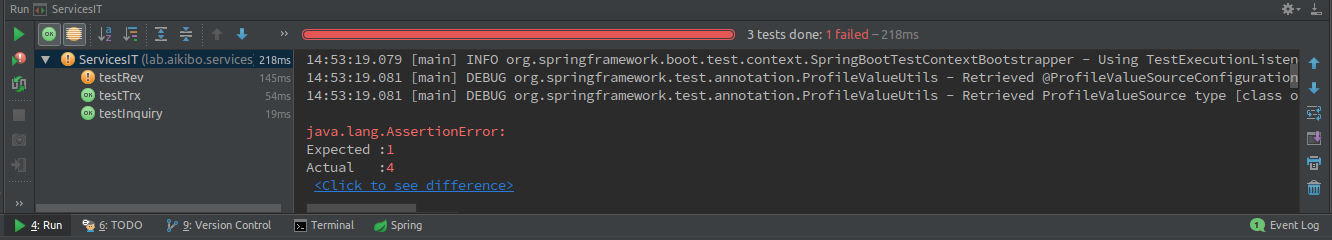
\includegraphics[width=1\textwidth]{./resources/07-services-it}
      \caption{Hasil \textit{Integration Test} Dengan Sistem Basis Data}
      \label{fig:services-it-fail}
    \end{figure}
    
    Terlihat bahwa ada kegagalan pada saat melakukan \texttt{testRev}, ini dikarenakan kode \texttt{NTPD} tidak sesuai atau tercatat pada basis data, maka diperlukan penyesuaian terhadap parameter \texttt{NTPD} yang sudah tercatat pada basis data pada pencatatan transaksi pembayaran sebelumnya, pada gambar \ref{fig:services-it-success} adalah hasil \textit{integration test} ke-2 setelah dilakukan penyesuaian terhadap parameter \texttt{NTPD}.
    
    \begin{figure}[H]
      \centering
      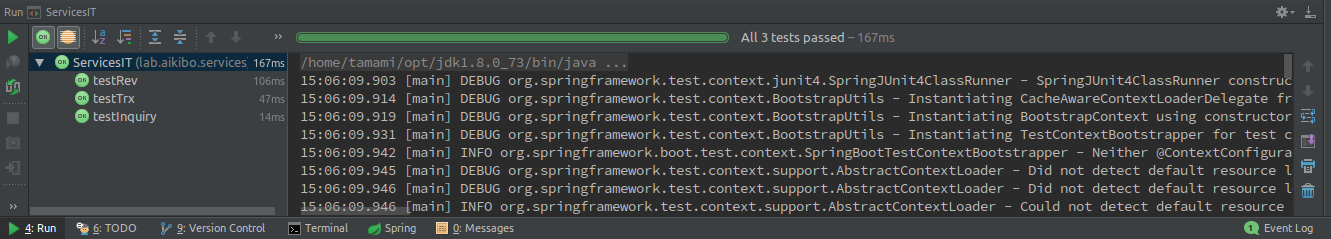
\includegraphics[width=1\textwidth]{./resources/08-services-it-2}
      \caption{Hasil \textit{Integration Test} Dengan Sistem Basis Data Ke-2}
      \label{fig:services-it-success}
    \end{figure}
    
  \end{enumerate}
\end{enumerate}


\section{KENDALA YANG DIHADAPI}

Kendala yang dihadapi pada saat melakukan \textit{unit test} tidak ada, hanya saja pada saat melakukan \textit{integration test}, dibutuhkan basis data model agar basis data aslinya tidak terpengaruh oleh kondisi \textit{test} yang merubah nilai dari isi basis data.


\section{KESALAHAN PROGRAM}

Kesalahan program yang ditemukan selama pengujian adalah pada saat memverifikasi kode mata anggaran untuk penerimaan pajak bumi dan bangunan, keputusannya apakah penerimaan pokok pajak dipisahkan mata anggarannya dengan denda administrasi pajak daerah.


\section{WAKTU PROSES UJI COBA}

Untuk proses uji cobanya sendiri sangat cepat, hanya kurang dari 1 jam, karena cukup melakukan eksekusi pada seluruh unit yang ada di dalam sistem aplikasi, dan melakukan eksekusi pada beberapa unit \textit{integration test}.


\end{document}